% =========================================================================== %

\begin{frame}[t,plain]
\titlepage
\end{frame}

% =========================================================================== %

\begin{frame}{Paths}
%
\begin{columns}
\column{.6\linewidth}
\begin{center}
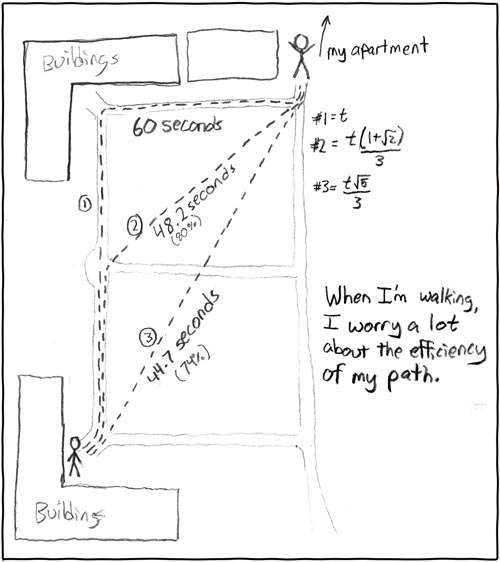
\includegraphics[width=0.6\linewidth]{./gfx/04-xkcd-paths}\\
\end{center}
%
\column{.2\linewidth}
\small
	\emph{It's true, I think about this all the time.}

	\vspace{6pt}
	\url{https://xkcd.com/85/}
\end{columns}
%
\end{frame}

% =========================================================================== %

\begin{frame}{Scope For Today}
%
\begin{itemize}
\item Numerical integration to find trajectories
	\begin{itemize}
	\item \texttt{scipy.integrate.solve\_ivp}
	\item Runge-Kutta-Integrator
	\item Leapfrog-Integrator
	\end{itemize}
\item Differential equations as eigenvalue problems
	\begin{itemize}
	\item \texttt{np.linalg.eig} and \texttt{eigh}
	\item \texttt{scipy.linalg.eigh\_tridiagonal} and similar optimizations
	\item Numerical stability
	\end{itemize}
\end{itemize}
%
\end{frame}

% =========================================================================== %

\begin{frame}{Solving Initial Value Problems}
%
\begin{itemize}
\item Scenario
	\begin{itemize}
	\item $y$ is an unknown function of form $ \mathbb{R} \to \mathbb{C}^{D}$
	\item Given: Function $f: \dv{t} y(t) = f(t, y)$
	\item Given: $y_0 = y(t_0)$
	\item Wanted: values $y_i = y(t_i)$ for arbitrary $t_i \in [t_0, t_N]$
	\end{itemize}
\item Solution
	\begin{itemize}
	\item \texttt{scipy.integrate.solve\_ivp}
	\item Most simple form: \texttt{result = solve\_ivp(f, [t\_0, t\_N], [y\_0])}
	\item \texttt{result} is of type \texttt{scipy.integrate.\_ivp.ivp.OdeResult}, which has attributes \texttt{t} and \texttt{y}
	\item \texttt{result.t} contains the $t_i$ as a Numpy array
	\item \texttt{result.y} contains the $y_i$ as a Numpy array
	\end{itemize}
\end{itemize}
%
\end{frame}

% =========================================================================== %

\begin{frame}[fragile]{A More Detailled Look At The Solver: The Function \texttt{f}}
%
\begin{itemize}
\item Callable
	\begin{itemize}
	\item May be a regular Python function (\inPy{def f(t, y): ...})
	\item May be a Lambda (\inPy{f = lambda t, y: ...})
	\item May be a class instance with a dunder call (\inPy{def __call__(self, t, y): ...})
	\end{itemize}
\item Parameters
	\begin{itemize}
	\item MUST accept parameters \texttt{t, y} in that oder
	\item Function body may ignore either or both of them
	\item May accept more parameters (we'll see later on)
	\item \texttt{t} -- time-like variable, \enquote{external} to the system
	\item \texttt{y} -- state-like variable, \enquote{the system at time \texttt{t}}
	\end{itemize}
\item Return Value
	\begin{itemize}
	\item $y'(t)$
	\item As a scalar if $y(t)$ is a scalar function
	\item As an iterable (\zB \inPy{list}, \inPy{tuple} or \inPy{np.array}), if $y(t)$ is a vector valued function
	\end{itemize}
\end{itemize}
%
\end{frame}

% =========================================================================== %

\begin{frame}[fragile]{A More Detailled Look At The Solver: Boundary Values}
%
\begin{itemize}
\item \texttt{t\_span} -- start and end time
	\begin{itemize}
	\item Two member sequence (\zB \inPy{list}, \inPy{tuple} or \inPy{np.array})
	\item SciPy decides on which points to evaluate in between
	\item Possible to set own evaluation points; must be present nonetheless
	\end{itemize}
\item \texttt{y0} -- initial value
	\begin{itemize}
	\item Must be a 1D sequence
	\item Scalars: just pass \texttt{[y\_0]}
	\item Vectors: just pass \texttt{y\_0}
	\item Fields: pass \texttt{field.reshape(field.size)} or \texttt{field.flatten()}
	\item Requires two extra \texttt{reshape}s in \texttt{f} (we'll see an example later on)
	\end{itemize}
\end{itemize}
%
\end{frame}

% =========================================================================== %

\begin{frame}[fragile]
%
\begin{codebox}[First Order ODE: $y' {=} \alpha \cdot t \cdot y$]
\begin{minted}[linenos, fontsize=\scriptsize]{python3}
y_0, alpha = 1.0, -0.2
t_min, t_max = 0, 10

f_prime = lambda t, y: alpha * t * y
result = scipy.integrate.solve_ivp(f_prime, [t_min, t_max], [y_0])
print(result)

times = np.linspace(t_min, t_max, t_N)
analytic_y = y_0 * np.exp(alpha * times ** 2 * 0.5)

plt.set_xlabel("t")
plt.set_ylabel("f(x, t)")
plt.set_title("Flat Projection of the Solution")
plt.plot(times, result.y[0], "o", label="numerical result")
plt.plot(times, analytic_y, "-", label="analytical result")
plt.legend()
plt.show()
\end{minted}
\end{codebox}
%
\end{frame}

% =========================================================================== %
%
\begin{frame}[fragile]
%
\begin{columns}
\column{.53\linewidth}
\begin{cmdbox}[Output: First Order ODE:  $y' {=} \alpha \cdot t \cdot y$]
\begin{minted}[fontsize=\scriptsize]{text}
  message: The solver successfully reached the 
           end of the integration interval.
  success: True
   status: 0
        t: [ 0.000e+00  2.000e-01 ...  
             9.800e+00  1.000e+01]
        y: [[ 1.000e+00  9.960e-01 ...  
              6.803e-05  4.581e-05]]
      sol: None
 t_events: None
 y_events: None
     nfev: 116
     njev: 0
      nlu: 0
\end{minted}
\end{cmdbox}
%
\column{.4\linewidth}
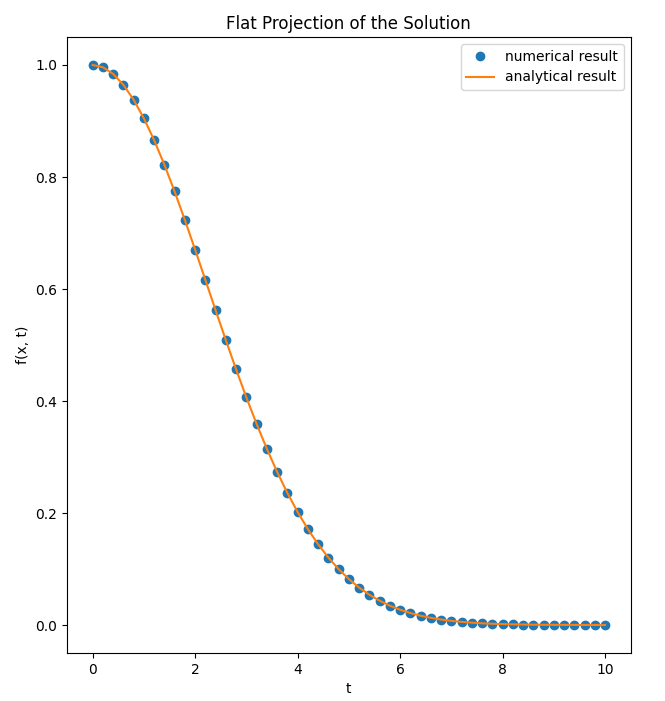
\includegraphics[width=\linewidth]{./gfx/04-ODE-solution}
\end{columns}
%
\vspace{-3pt}
\begin{hintbox}[Attributes of \texttt{result}]
\footnotesize
You can access each of the displayed elements of \texttt{result} via \texttt{result.attribute}, \zB \texttt{result.sccess} to check whether or not your simulation could be completed.
\end{hintbox}
%
\end{frame}

% =========================================================================== %

\begin{frame}{Some Optional Parameters To \texttt{solve\_ivp}}
%
\begin{itemize}
\item  \texttt{t\_eval}: \inPy{list} or \texttt{np.array} of times at which to evaluate
	\begin{itemize}
	\item \texttt{solve\_ivp(f, [t0, tX], [y0], t\_eval=[t0, t0 + delta\_t, tX])}
	\item Need not be within \texttt{[t0, tX]}
	\item Only affects what is stored
	\item Usually needed to produce nice-looking plots
	\item Often: \texttt{np.arange} or \texttt{np.linspace}
	\end{itemize}
\item \texttt{args}: \inPy{tuple} of arbitrary values
	\begin{itemize}
	\item Passed on to \texttt{f} after the \texttt{t, y} parameters
	\item Example: \inPy{f = lambda t, y, alpha: alpha * t * y}
	\item Call: \texttt{solve\_ivp(f, [t0, tX], [y0], args=(0.2,))}
	\item Note the comma -- Python's way of distinguishing between \inPy{tuple}s and expressions in parentheses
	\end{itemize}
\item \texttt{method}: \inPy{str}ing, specifying the integration method
	\begin{itemize}
	\item More details on the next couple of slides
	\end{itemize}
\item \texttt{vectorized}: \inPy{bool}ean, telling whether to allow some optimizations
\end{itemize}
%
\end{frame}

% =========================================================================== %

\begin{frame}{How Does It Do That -- Runge-Kutta-Methods}
%
\begin{itemize}
\item Problem: computation time vs. accuracy
	\begin{itemize}
	\item Could use integrators's we've seen last week (Romberg, Simpson, ...)
	\item High cost as they need several points in between
	\item Additional floating point errors as $\varepsilon$ gets very small
	\end{itemize}
\item Solution: cheap algorithm with non-fixed $\varepsilon$
	\begin{itemize}
	\item When $\dv{t} y(t) \approx const \Leftrightarrow \dv[2]{t} y(t) \approx 0$: few points in between (\enquote{$\varepsilon$ big})
	\item Increase number of sampling points (\enquote{$\varepsilon$ smaller}) in \enquote{interesting} sections
	\end{itemize}
\item Runge-Kutta-Methods: variants of Euler's Method
	\begin{itemize}
	\item Euler: $y_{t + \varepsilon} = y_t + y'_t \cdot \varepsilon$
	\item Vary $\varepsilon$ as function of $y''_t$
	\item Extra accuracy with some in-between points
	\end{itemize}
\end{itemize}
%
\begin{hintbox}[Notation]
\scriptsize
In the literature, you'll often find the symbol $h$ in lieu of $\varepsilon$. That's mostly because codes are often limited to the ASCII space (not so in Python) and typing roman letters is more convenient than using unicode symbols. The choice of $h$ comes from the word \emph{height}.
\end{hintbox}
%
\end{frame}

% =========================================================================== %

\begin{frame}{Runge-Kutta-Methods of Order $N$}
%
\begin{columns}
\column{.5\linewidth}
\begin{itemize}
\item Use $N$ intermediate estimates for $y'(t)$, usually denoted as $k_i$
	\begin{itemize}
	\item Evaluated partially at \enquote{in-between time points} $t_i + \beta \varepsilon$ with $\beta \in (0, 1)$
	\end{itemize}
\item Runge-Kutta Order 4 (RK4)
	\begin{itemize}
	\item $f_1 = f(t_n, y_n)$
	\item $f_2 = f(t_n + \sfrac{\varepsilon}{2}, y_n + \sfrac{\varepsilon}{2} k_1$
	\item $f_3 = f(t_n + \sfrac{\varepsilon}{2}, y_n + \sfrac{\varepsilon}{2} k_2$
	\item $f_4 = f(t_n + \varepsilon, y_n + \varepsilon k_3$
	\item[\Thus] $y_{n+1} = y_n + \sfrac{\varepsilon}{6}(k_1 + 2k_2 + 2k_3 + k_4)$
	\item[\Thus] Error in $\mathcal{O}(\varepsilon^4)$
	\end{itemize}
\item SciPy-Default
	\begin{itemize}
	\item RK5 to get the points
	\item RK4 to control magnitude of $\varepsilon$
	\end{itemize}
\end{itemize}
%
\column{.4\linewidth}
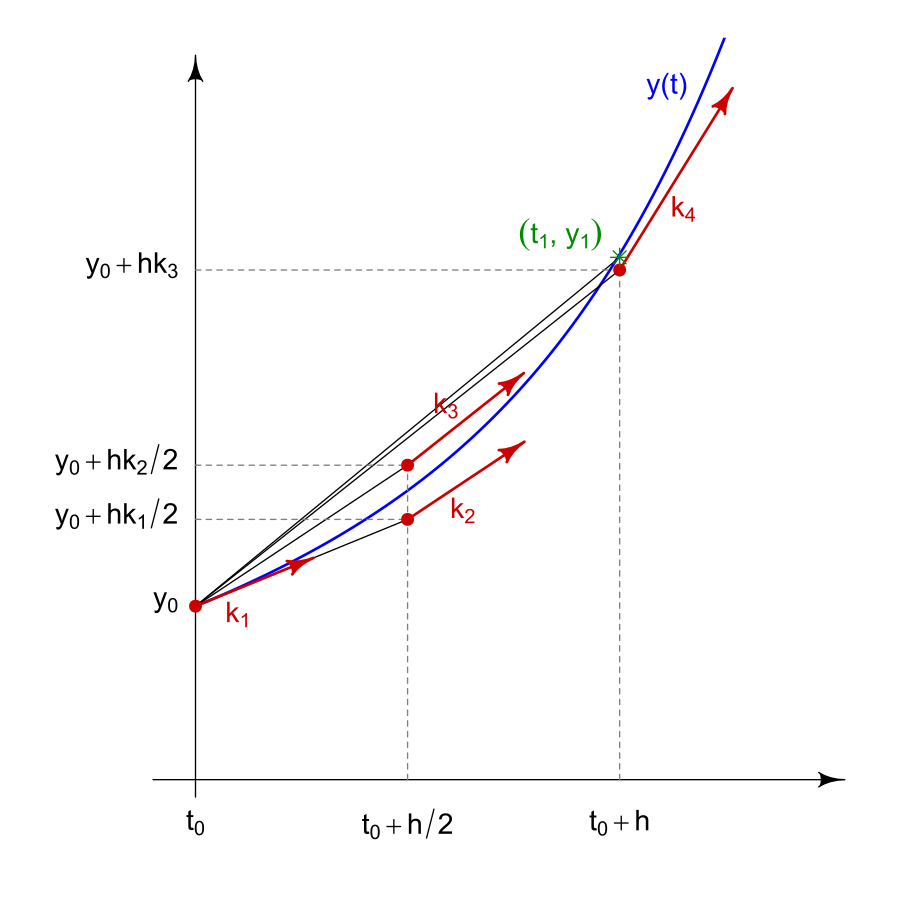
\includegraphics[width=\linewidth]{./gfx/04-Runge-Kutta}

\scriptsize
Image by Wikipedia-User HilberTraum\\
\url{https://en.wikipedia.org/wiki/File:Runge-Kutta_slopes.svg}
\end{columns}
%
\end{frame}

% =========================================================================== %

\begin{frame}{Second Order and Higher Order ODEs}
%
\begin{itemize}
\item Remember: \texttt{solve\_ivp} can handle vector valued ODEs
\item From $y(t)$, construct a vector $\vec{v}(t)$ with $v_i(t) = y^{(i-1)}(t)$
	\begin{itemize}
	\item E.\;g. third order ODE: $
		\vec{v}(t) = 
		\begin{pmatrix}
			y(t) \\
			y'(t) \\
			y''(t)
		\end{pmatrix}$
	\item Result: you can express the entire system in terms of first order derivatives:\\
		$\dv{t} v_i(t) = y^{(i)}(t)$
	\item E.\;g. $
		\dv{t} \vec{v}(t) = 
		\begin{pmatrix}
			y'(t) \\
			y''(t) \\
			f(t, y)
		\end{pmatrix}$
	\end{itemize}
\end{itemize}
%
\begin{hintbox}[Useful function]
\footnotesize
The function \texttt{np.roll(array, offset)} is useful for this. It returns a permutation of \texttt{array}, which is shifted by \texttt{offset} to the right. So, if \texttt{offset == -1}: \texttt{[0, 1, 2, 3]} \thus \texttt{[1, 2, 3, 0]}. Overwrite the last component with \texttt{f(t, y)}, and you've constructed your result vector!
\end{hintbox}
%
\end{frame}

% =========================================================================== %

\begin{frame}[fragile]
%
\begin{codebox}[Second Order ODE: $y'' {=} \cos(t)$]
\begin{minted}[linenos, fontsize=\scriptsize]{python3}
y_0 = -1
v_0 = +0
f_prime = lambda t, y: (y[-1], np.cos(t))

t_min = 0
t_max = 10
times = np.linspace(t_min, t_max, 51)

result = scipy.integrate.solve_ivp(f_prime, [t_min, t_max], [y_0, v_0], t_eval=times)

positions = result.y[0, :]
velocities = result.y[1, :]

plt.title("$y''(t) = \cos(t)$")
plt.plot(times, positions, label="y(t): positions")
plt.plot(times, velocities, label="y'(t): velocities")
plt.legend()

plt.show()
\end{minted}
\end{codebox}
%
\end{frame}

% =========================================================================== %

\begin{frame}{Result and Notes}
%
\begin{columns}
\column{.6\linewidth}
\begin{itemize}
\item You can also invert the order of derivatives, \ie $v_i(t) = y^{(D-i)}(t)$ (or any order you fancy)
\item Order of derivatives in \texttt{result} matches order in \texttt{f(t, y)}
\item Of course, so does order in \enquote{initial state} vector
\item Making index match order is a nice way to save on mental load.
\end{itemize}
%
\column{.4\linewidth}
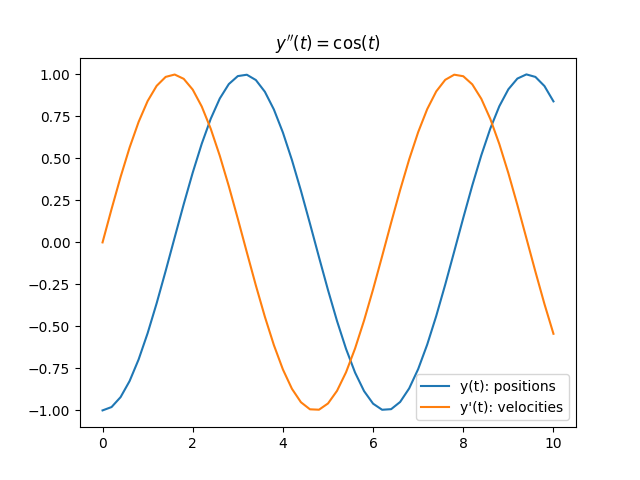
\includegraphics[width=\linewidth]{./gfx/04-ODE-second-degree}
\end{columns}
%
\begin{hintbox}[Vector Valued Higher Order ODEs]
\footnotesize
You can also do vector valued higher order ODEs with the same trick (pack everything into one vector)
\end{hintbox}
%
\end{frame}

% =========================================================================== %

\begin{frame}{Scalar and Vector Field ODEs}
%
\begin{itemize}
\item \texttt{solve\_ivp} requires \texttt{y\_0} to be 1-dimensional vector
\item NumPy-Arrays \emph{of any dimension} are just 1-dimensional structures in memory
	\begin{itemize}
	\item Python-object model: class \texttt{numpy.ndarray} stores \texttt{shape} information separate from \texttt{data}
	\item \texttt{shape} can be changed without affecting the \texttt{data}
	\item \texttt{array.reshape(new\_shape)} and \texttt{array.flatten} do the trick
	\end{itemize}
\item Before calling \texttt{solve\_ivp}:
	\begin{itemize}
	\item \texttt{y\_0 = field.reshape(field.size)} or \texttt{y\_0 = field.flatten()}
	\end{itemize}
\item In \texttt{f(t, y)}:
	\begin{itemize}
	\item \texttt{locally\_reconstructed = y.reshape(old\_shape)}
	\item Compute derivative on \texttt{locally\_reconstructed}
	\item \inPy{return locally_reconstructed.flatten()}
	\end{itemize}
\item Vector valued fields are just $N+1$ dimensional scalar fields$^{*}$\\
 {\scriptsize($^{*}$ with a discrete $N+1^{\text{st}}$ dimension)}
\end{itemize}
%
\end{frame}

% =========================================================================== %

\begin{frame}[fragile]{Example: Laplace Equation}
%
\begin{itemize}
\item Laplace Equation: $\laplacian \phi = 0$
	\begin{itemize}
	\item Usually: Dirichlet boundary conditions $\eval{y(\vec{r})}_{\partial\Omega}$ is known
	\item Also possible: Neumann boundary conditions, $\eval{y'(\vec{r})}_{\partial\Omega}$ (\emph{derivative}) is known
	\item ... and any combination of initial values that fix all degrees of freedom
	\end{itemize}
\item Approach: Self Consistent Field (SCF)
	\begin{itemize}
	\item Compute correction operator and deduce change
		\begin{itemize}
		\item Correction operator, here: $(\laplacian - \rho)\phi$
		\item $\rho$ is just the right hand side of the differential equation (\ie $0$ in our case)
		\end{itemize}
	\item Iterate until it converges (changes by less than some $\varepsilon$)
	\item Works because result of correction operator has correct sign and becomes zero if correct result is realized
	\end{itemize}
\item Set derivative to zero on boundary values \Thus \emph{fixed} values
\end{itemize}
%
\end{frame}

% =========================================================================== %

\begin{frame}[fragile]
%
\begin{codebox}[Laplace Equation (1)]
\begin{minted}[linenos, fontsize=\scriptsize]{python3}
# prepare the Laplace operator (convolution kernel)
laplacian = np.zeros((3, 3), dtype=np.float)
laplacian[1, :] = +1
laplacian[:, 1] = +1
laplacian[1, 1] = -4

# prepare our potential field -- random values
size_x = 50
size_y = 50
shape = (size_y, size_x)
field = np.random.random(shape)

# but set the known boundary values
field[+0, :] = 0  # top row
field[-1, :] = 1  # bottom row

# lazy convergence spec: compute fixed amount of steps
t_min = 0
t_max = 200                         # this encodes our convergence limit
t_eval = [10, t_max]                # this will be used later for plots
\end{minted}
\end{codebox}
%
\end{frame}

% =========================================================================== %

\begin{frame}[fragile]
%
\begin{codebox}[Laplace Equation (2)]
\begin{minted}[linenos, firstnumber=last, fontsize=\scriptsize]{python3}
def f_prime(t, y, shape, laplacian):
    y = y.reshape(shape)

    dy = scipy.signal.convolve(y, laplacian, mode='same')
    dy[+0, :] = 0  # top row
    dy[-1, :] = 0  # bottom row

    return dy.reshape(y.size)

result = scipy.integrate.solve_ivp(f_prime, [t_min, t_max],
                                   field.reshape(field.size),
                                   args=(shape, laplacian),
                                   t_eval=t_eval)
print(result)
\end{minted}
\end{codebox}
%
\end{frame}

% =========================================================================== %

\begin{frame}[fragile]
%
\begin{codebox}[Laplace Equation (3)]
\begin{minted}[linenos, firstnumber=last, fontsize=\scriptsize]{python3}
fig, axs = plt.subplots(2, 3)
fig.set_size_inches(15, 10)
fig.suptitle("Solution to $\Delta \phi = 0$ with boundary conditions")

for row_id, time in enumerate(t_eval):
    final_field = result.y[:, row_id].reshape(shape)
    laplacian_values = scipy.signal.convolve(final_field, laplacian)
    forces_y, forces_x = np.gradient(final_field)   # sic: order is y, x here
    grid_y, grid_x = np.indices(shape)              # ... and here, too

    # ... some matplotlib code -- see GRIPS

plt.show()
\end{minted}
\end{codebox}
%
\begin{hintbox}[Finding the correct index]
\footnotesize
Indices never come intuitively to me. Sometimes, results are appended in a first-index fashion, sometimes (like here) it's on the last index.
In development, typing \inPy{print(result.y.shape)} often gives you a valuable hint which index contains \enquote{your} information.
\end{hintbox}
%
\end{frame}

% =========================================================================== %

\begin{frame}
%
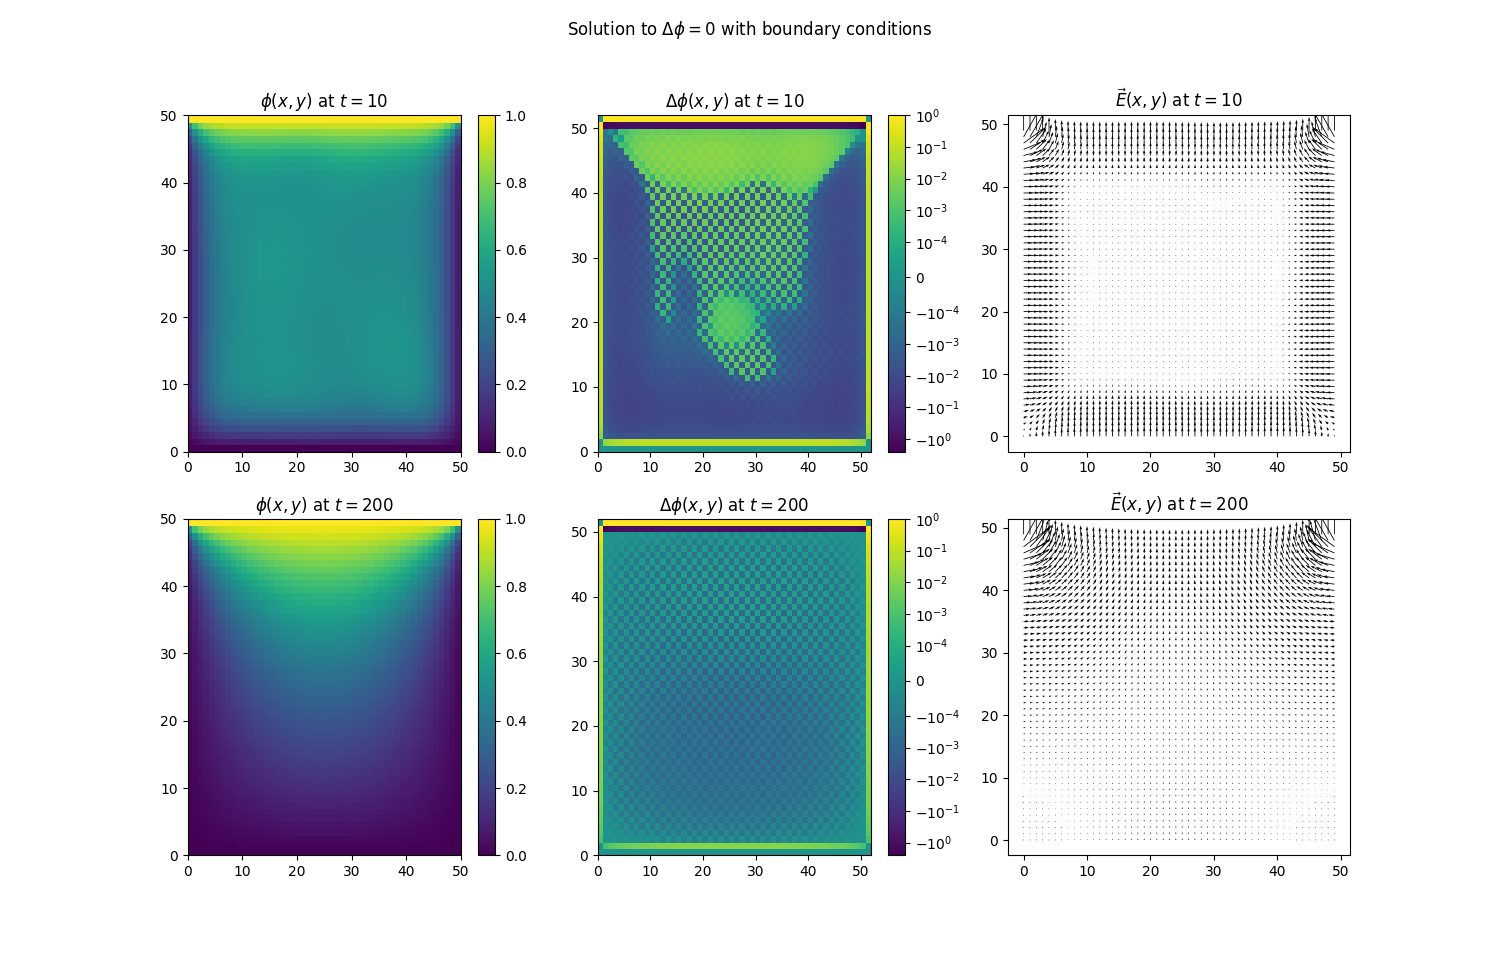
\includegraphics[width=\linewidth]{./gfx/04-Laplacian}
%
\end{frame}

% =========================================================================== %

\begin{frame}[fragile]
%
\begin{columns}
\column{.72\linewidth}
\begin{codebox}[Orbital Mechanics]
\begin{minted}[linenos, fontsize=\scriptsize]{python3}
def f_prime(t, y, shape, laplacian):
    position = y[:2]
    distance_factor = np.sum(position ** 2) ** (3 / 2)
    accelereation = -(G * m_sun / distance_factor) * position

    result = np.roll(y, -2)
    result[2:] = accelereation

    return result

result = scipy.integrate.solve_ivp(
    f_prime,
    [t_min, t_max], 
    [*r_planet, *v_planet],
    t_eval=times,
    method=method
)
\end{minted}
\end{codebox}
%
\column{.3\linewidth}
\begin{itemize}
\item Central object of mass \texttt{m\_sun}
\item Force between objects: $F = G \cdot \dfrac{m_{\text{sun}} m_{\text{planet}}}{r^2}$
\item Force is vector valued, always points towards sun\\
	\Thus extra factor $-\dfrac{\vec{r}}{r}$
\item $\vec{a} = \dfrac{\vec{F}}{m}$ \\
	\Thus no \texttt{m\_planet}
\item $\vec{y} = 
	\begin{pmatrix}
	r_x \\ r_y \\ v_x \\ v_y
	\end{pmatrix}$
\end{itemize}
\end{columns}
%
\end{frame}

% =========================================================================== %

\begin{frame}
%
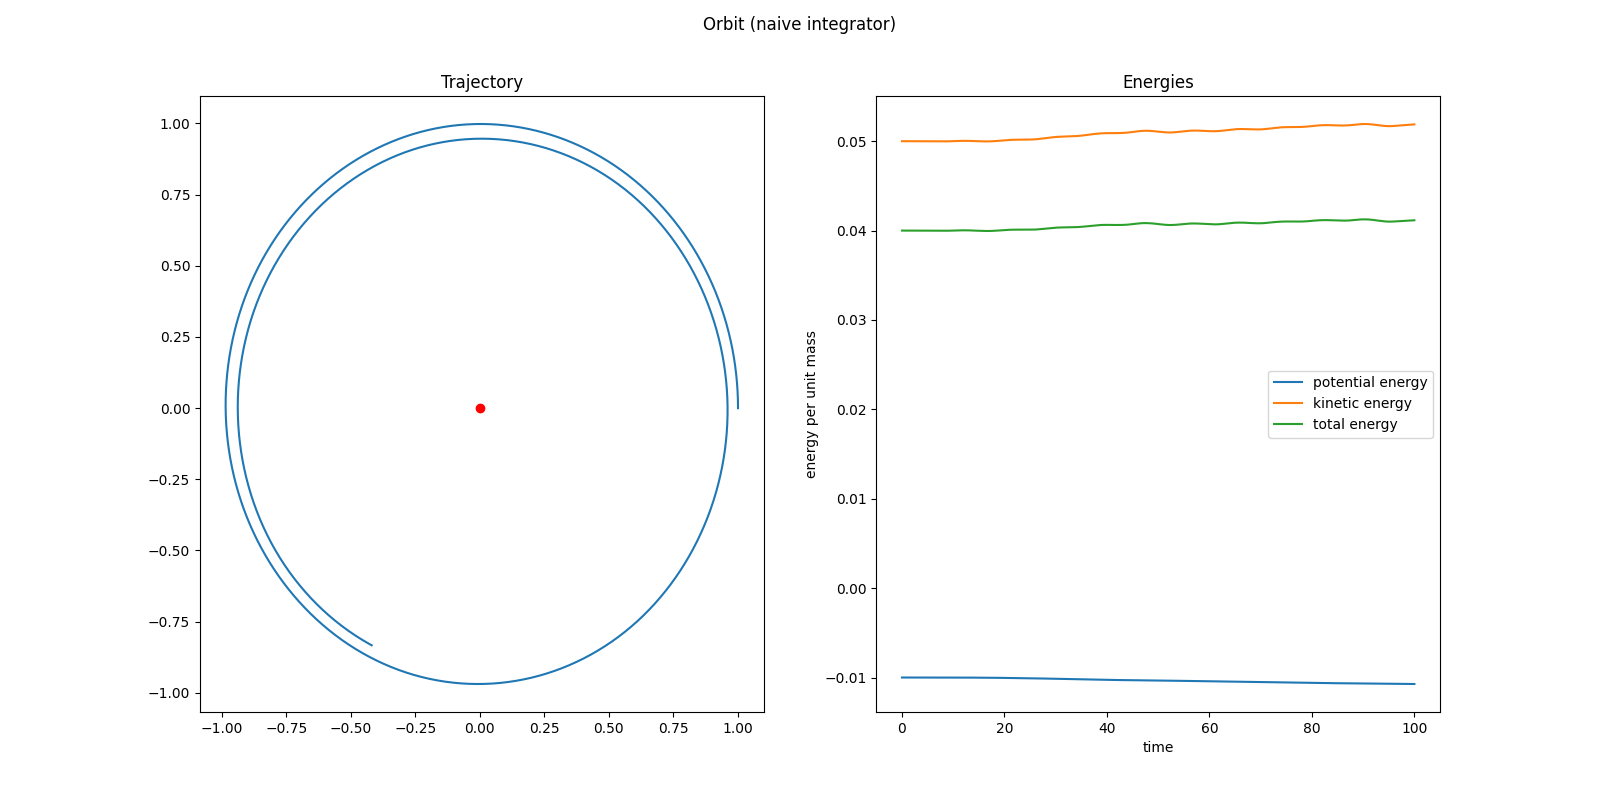
\includegraphics[width=\linewidth]{./gfx/04-orbital-mechanics}

\begin{center}
\emph{\enquote{Oh shit.}}
\end{center}
%
\end{frame}

% =========================================================================== %

\begin{frame}{Time Reversibility and Leapfrog Integrator}
%
\begin{itemize}
\item Energy drift of 2$^{\text{nd}}$ and higher order ODEs is a known problem
\item Root cause: used integration method not time reversible
	\begin{itemize}
	\item Integrator (= RK45) sees different forces when going forward or backward in time
	\item Other explanation
		\begin{itemize}
		\item Positive curvature of potential: travelled distance under-estimated 
			\Thus stays longer in \enquote{pumping} region
		\item Negative curvature of potential: travelled distance over-estimated
			\Thus leaves \enquote{draining} region earlier
		\end{itemize}
	\end{itemize}
\item Solution: time reversible integrators
\item In particular: Leapfrog integration
	\begin{itemize}
	\item Compute acceleration as usual: $a_i = \sfrac{1}{m} \; f(t, y)$
	\item \emph{Half time} steps for velocity: $v_{i + \mathbf{\sfrac{1}{2}}} =
		v_{i - \mathbf{\sfrac{1}{2}}} +
		a_i \varepsilon$
	\item Position steps at integer times with half-time velocities: $x_{i+1} = x_i + v_{i + \mathbf{\sfrac{1}{2}}} \varepsilon$
	\end{itemize}
\item For an example and more details, see \url{http://cvarin.github.io/CSci-Survival-Guide/leapfrog.html} 
\end{itemize}
%
\end{frame}

% =========================================================================== %

\begin{frame}{Eigensystems}
%
\begin{itemize}
\item Let there be a differential operator $\mathcal{D}$
\item Ask for spectrum: $\mathcal{D}f(x) = \lambda f(x)$
	\begin{itemize}
	\item Niche problems like in $\mathcal{D} = -\dfrac{\hbar^2}{2m} \laplacian + V(x)$
	\item[\Thus] Not only function $f$ but also eigenvalue $\lambda$
	\end{itemize}
\item Numpy and SciPy: submodules for linear algebra
	\begin{itemize}
	\item \texttt{numpy.linalg.eig} and \texttt{numpy.linalg.eigh} (general and hermitean matrices)
	\item \texttt{scipy.linalg.eig} and \texttt{scipy.linalg.eigh} for \emph{generalized} eigenvalue problems
	\item \texttt{scipy.linalg.eig\_banded} and \texttt{scipy.linalg.eigh\_tridiagonal} (optimized for sparse matrices)
	\end{itemize}
\item We can use them without any basis transformation!
	\begin{itemize}
	\item All we need to do is to formulate $\mathcal{D}$ as a discrete operator on real space
	\item It's easy, I promise
	\end{itemize}
\end{itemize}
%
\end{frame}

% =========================================================================== %

\begin{frame}{Formulating a Differential Operator}
%
\begin{itemize}
\setlength\itemsep{3pt}
\item Remember discretization rule: $\dv[2]{x}f(x) \to \dfrac{f_{i-1} - 2f_i + f_{i+1}}{\varepsilon^2}$
\item Which gave us the convolution kernel $\mathcal{K} = \sfrac{1}{\varepsilon^2}
\begin{pmatrix}
1 & -2 & 1
\end{pmatrix}
$
\item Which is used in $f''_i = \sum_{j=1}^{3} f_{i+j} \; \mathcal{K}_j$
\item Looks a bit like a matrix multiplication, doesn't it?
	\begin{itemize}
	\setlength\itemsep{2pt}
	\item Remember: $(AB)_{ij} = \sum_k A_{ik} \; B_{kj}$
	\item Dot product between $i^{\text{th}}$ row of $A$ and $j^{\text{th}}$ column of $B$
	\item Convolution: dot product between $\mathcal{K}$ and subvector of $f$
	\item Pad $\mathcal{K}$ with some zeros to be compatible with matrix multiplication formalism without changing result
	\item Repeat for different positions $i$
	\end{itemize}
\end{itemize}
%
\end{frame}

% =========================================================================== %

\begin{frame}{Formulating a Differential Operator}
%
\vspace{-6pt}
\begin{align*}
	\dv[2]{x}
&\to
	\dfrac{1}{\varepsilon^2}
	\begin{pmatrix}
		&&\ddots \\
		0 & \ldots & +1 & -2 & +1 & 0 & 0 & \ldots & 0 \\
		0 & \ldots & 0 & +1 & -2 & +1 & 0 & \ldots & 0 \\
		0 & \ldots & 0 & 0 & +1 & -2 & +1 & \ldots & 0 \\
		&&&&&&\ddots 
	\end{pmatrix}
\end{align*}
%
\vspace{-3pt}
\begin{itemize}
\item First and last line:
	\begin{itemize}
	\item Cyclic boundary conditions: $
		\begin{pmatrix}
		-2 & +1 & 0 & \ldots & 0 & \mathbf{+1}
		\end{pmatrix}
		$
	\item Forward definition: $
		\begin{pmatrix}
		\mathbf{+1} & -2 & +1 & 0 & \ldots & 0 & 0
		\end{pmatrix}
		$
	\item \enquote{Yolo}: $
		\begin{pmatrix}
		-2 & +1 & 0 & \ldots & 0 & 0
		\end{pmatrix}
		$ \\
		(Just accept that the first and last value will be off)
	\item (Last lines analogously)
	\end{itemize}
	\item Add $V(x_i)$ to the principal diagonal and you've got $\mathcal{D}$!
\end{itemize}
%
\end{frame}

% =========================================================================== %

\begin{frame}[fragile]
%
\begin{codebox}[Eigensystem: Free Particle (Unscaled)]
\begin{minted}[linenos, fontsize=\scriptsize]{python3}
resolution = 200

principal_diagonal = -2 * np.ones(resolution    , dtype=np.float64)
secondary_diagonal = +1 * np.ones(resolution - 1, dtype=np.float64)
matrix = np.diag(principal_diagonal) + \
         np.diag(secondary_diagonal, -1) + \
         np.diag(secondary_diagonal, +1)

eigenvalues, eigenvectors = np.linalg.eigh(matrix)
# eigenvalues, eigenvectors = scipy.linalg.eigh_tridiagonal(principal_diagonal, 
#                                                           secondary_diagonal)
xs = np.linspace(0, 2 * np.pi, resolution)
for excitation in range(4):
    plt.plot(xs, eigenvectors.T[excitation], label=f"excitation #{excitation}")
plt.legend(loc="lower left")
plt.show()
\end{minted}
\end{codebox}
%
\end{frame}

% =========================================================================== %

\begin{frame}{Free Particle (Unscaled)}
%
\begin{columns}
\column{.5\linewidth}
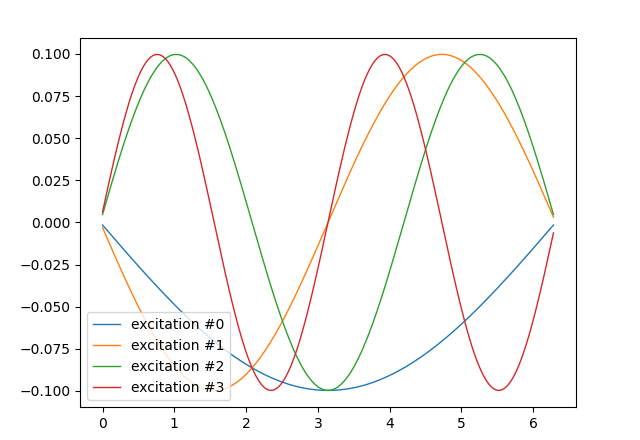
\includegraphics[width=\linewidth]{./gfx/04-free-particle-success}
%
\column{.5\linewidth}
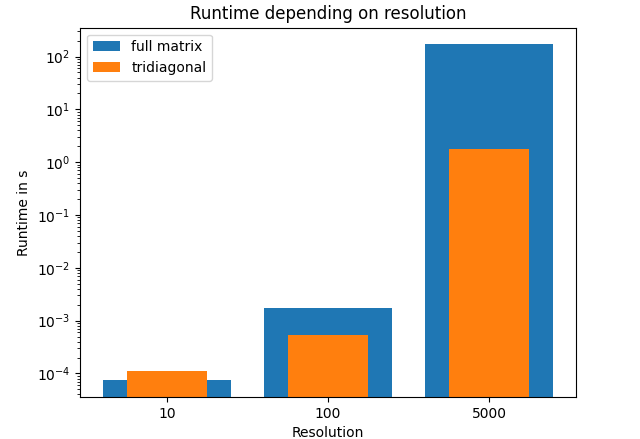
\includegraphics[width=\linewidth]{./gfx/04-free-particle-runtime}
\end{columns}
%
\begin{hintbox}[Overall Runtime Behaviour]
\footnotesize
Eigensystem-Algorithms are usually in $\mathcal{O}(N^3)$. Sparse-matrix solvers are usually in a better time complexity class like $\mathcal{O}(N^2)$ or even $\mathcal{O}(N \log(N))$.
\end{hintbox}
%
\end{frame}

% =========================================================================== %

\begin{frame}{Free Particle (Unscaled) -- Actual Plot}
%
\begin{columns}
\column{.5\linewidth}
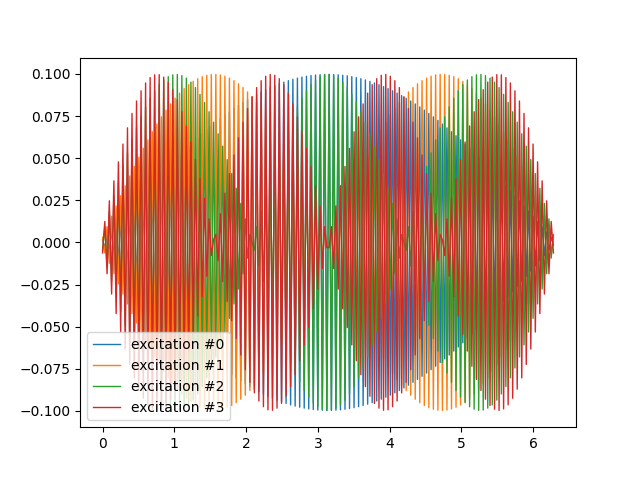
\includegraphics[width=\linewidth]{./gfx/04-free-particle-fail}
%
\column{.5\linewidth}
\begin{itemize}
\item Eigenvalues/Eigenvectors automatically sorted
	\begin{itemize}
	\item Smallest to biggest
	\end{itemize}
\item $Ax = \lambda x \Thus A(-x) = -\lambda x$
	\begin{itemize}
	\item Numerical instabilities can \enquote{flip} the eigenvectors
	\item Produces sign-flipped eigenvalues
	\end{itemize}
\item Recreate proper order
	\begin{itemize}
	\item \texttt{order = np.abs(evals).argsort()}
	\item \texttt{evecs = evecs[:, order]}
	\item Only for all free/positive or all bound/negative eigenvalues
	\item Otherwise: more creative sorting method
	\item E.\;g. by evaluating an operator on the function
	\end{itemize}
\end{itemize}
\end{columns}
%
\end{frame}

% =========================================================================== %

\begin{frame}[fragile]{Tangent: Evaluating an Operator on a Discretized Function}
%
\begin{itemize}
\item Let there be an non-differential operator $\mathcal{A}$
	\begin{itemize}
	\setlength\itemsep{3pt}
	\item Mathematically: $\mathcal{A}: \mathcal{A}(x, f) -> a(x)$
	\item E.\;g. potential operator $\hat{V}: \eval{\hat{V} \psi}_{x} = V(x) \psi(x)$
	\item Python: callable with signature like \inPy{A = lambda x_i, f_i : ... # returns scalar}
	\item E.\;g. potential operator \inPy{A = lambda x_i, f_i : potential(x_i) * f_i}
	\end{itemize}
\item Then $\matrixel{\psi}{\mathcal{A}}{\psi}$ can be transcribed to python very easily
	\begin{itemize}
	\item \inPy{np.sum(A(x, eigenvector[:, excitation]) * dx}
	\end{itemize}
\item For differential operators
	\begin{itemize}
	\item Like $\mathcal{A} = \alpha \dv{x}$
	\item Write operator as convolution kernel: \texttt{A = alpha * np.array([1, -2, 1])}
	\item Integrate with numpy: \inPy{np.sum(convolve(A, eigenvector[:, excitation], mode='same')) * dx}
	\item \inPy{mode='same'} leaves out the boundary values which are probably BS anyway
	\end{itemize}
\end{itemize}
%
\end{frame}

% =========================================================================== %

\begin{frame}{Free Particle Results}
%
\begin{columns}[T]
\column{=.5\linewidth}
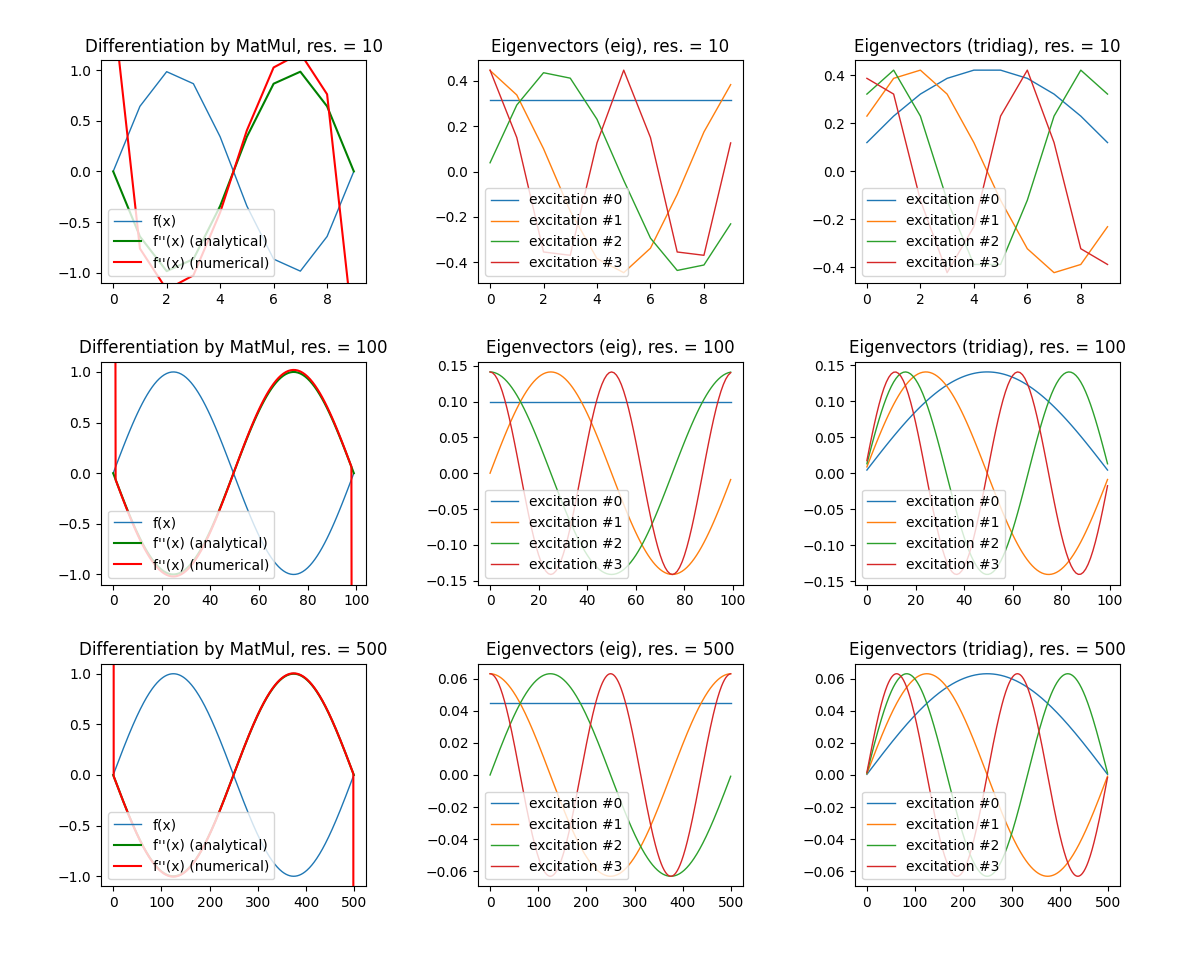
\includegraphics[width=\linewidth]{./gfx/04-free-particle-resolutions}
%
\column{=.4\linewidth}
\begin{itemize}
\item Operator $\mathcal{D} = \dv[2]{x}$
\item Left column: 
	\begin{itemize}
	\item \texttt{D @ y} 
	\item \texttt{y = np.sin(np.linspace(0, 2*np.pi, resolution)}
	\item No noteworthy deviation from analytical result for reasonable resolutions
	\item Except for boundary values
	\item (Cyclical boundary conditions)
	\item (Forward/Backward def would be better here, but not good)
	\end{itemize}
\item Other columns: Eigenvectors
\end{itemize}
\end{columns}
%
\end{frame}

% =========================================================================== %

\begin{frame}{Particle in Harmonic Potential}
%
\begin{center}
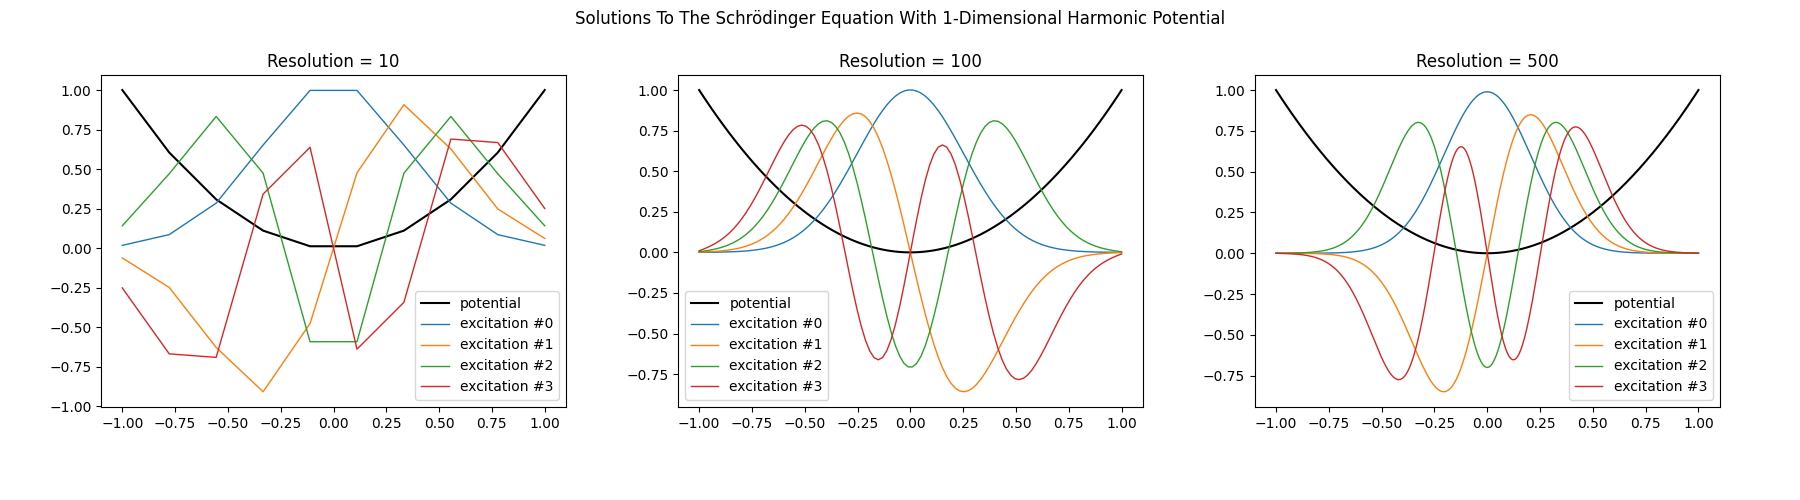
\includegraphics[width=\linewidth]{./gfx/04-harmonic-osciallator}
\end{center}
%
\begin{hintbox}[Code on GRIPS]
\footnotesize
As always, you'll find the code that produced these plots on GRIPS. Feel free to toy around with them!
\end{hintbox}
%
\end{frame}

% =========================================================================== %

\begin{frame}{Useful Tips When Dealing With Eigenvalue Problems}
%
\small
\begin{itemize}
\item If possible use the sparse matrix solvers like \texttt{eigh\_tridiagonal}
	\begin{itemize}
	\item Faster, less memory consumption \emph{and more accurate}
	\item Memory consumption for a full matrix is i $\mathcal{O}(N^2)$, while for sparse matrices it is often in $\mathcal{O}(N)$
	\item 8 Byte per real number, 16 bytes per complex number
	\end{itemize}
\item Avoid rescaling the matrix elements
	\begin{itemize}
	\item Often creates very small/large values ($\propto \hbar^2$), which gives numerics issues
	\item In particular, omit the $\sfrac{1}{\varepsilon^2}$ prefactor (rescale potential by $\varepsilon^2$ instead)
	\item Rescale eigenvectors after computing them
	\item Always do qualitative code without scaling factors first to know your method is working in the first place!
	\end{itemize}
\item Recipe can also be used for multidimensional eigenvalue problems
	\begin{itemize}
	\item Operator matrix will then be banded, not tridiagonal
	\item Use \texttt{matrix.strides} and \texttt{matrix.itemsize} to find the displacement between the bands
	\end{itemize}
\end{itemize}
%
\end{frame}

% =========================================================================== %